%%%%%%%%%%%%%%%%%%%%%%%%%%%%%%%%%%%%%%%%%%%%%%%%%%%%%%%
\subsection{Efficient Deployment}
\label{sec:efficient-deployment}
%%%%%%%%%%%%%%%%%%%%%%%%%%%%%%%%%%%%%%%%%%%%%%%%%%%%%%%

This benchmark tests the impact of optimisations to reduce build time of spack stacks described in~\sect{sec:faster-builds}, namely building in memory and caching previously-built packages.

For this demonstration, we built a software stack that has all of the dependencies required to develop Arbor~\cite{paper:arbor2019,software:arbor}, a Neuroscience application written in C++ and Python.
Arbor has a extensive list of dependencies, including C++ libraries, Python and Python packages.

We time the time taken to run make on a clean build, which includes the time taken to bootstrap Spack, concretise and build all of the packages and generate the compressed SquashFS image in four different scenarios:
\begin{itemize}
    \item \textbf{scratch}: Build on an HPE Cray ClusterStor E1000 Scratch file system.
    \item \textbf{memory}: Build in \lst{/dev/shm}, i.e. \emph{in memory}.
    \item \textbf{cache}: Build in \lst{/dev/shm} using a Spack build cache that has all of the packages 
    \item \textbf{partial}: Build in \lst{/dev/shm} using a Spack build cache where the version of Python in the recipe is changed to a version that is not in the cache.
\end{itemize}
Scenario 2 quantifies the effect of building in memory, and scenarios 3 and 4 illustrate the additional benefits of using build caches.

\begin{figure}[htp!]
    \begin{center}
        \begin{tikzpicture}[scale=1]
    \begin{axis} [
        ymin = 0, ymax=3000,
        ybar, bar width = 18pt,
        %symbolic x coords={1,2,3,4},
        grid=major,
        xtick = {1,2,3,4},
        xticklabels = {scratch, memory, cache, partial},
        xticklabel style={text height=1ex},
        ylabel={Build time (s)},
        nodes near coords,
        nodes near coords style={fill=white},
    ]
        \addplot[fill=orange!30] table[x=id, y=time-s] {./data/stack-build.tbl};
        \draw[line width=2pt, ->] (axis cs:2,2714) -- (axis cs:2,1866);
        \draw[line width=2pt, ->] (axis cs:3,1566) -- (axis cs:3,445);
        \draw[line width=2pt, ->] (axis cs:4,1566) -- (axis cs:4,787);
        \node[fill=white] () at (axis cs:2,2300) {\bfseries 1.7x};
        \node[fill=white] () at (axis cs:3,1000) {\bfseries 10.8x};
        \node[fill=white] () at (axis cs:4,1200) {\bfseries 3.2x};

        %\draw (s1_t.center) -- (s1_b.center);
    \end{axis}
\end{tikzpicture}


    \end{center}
    \caption{Reduction in time to build a complete Spack stack when building in memory and using Spack build caches compared with building on the scratch filesystem.}
    \label{fig:image-build}
\end{figure}

\fig{fig:image-build} shows that building the image on Scratch takes 45 minutes, which is reduced to 26 minutes when building in memory -- a significant 1.7$\times$ reduction in build time.
Less than 3 minutes are required when all packages are available in a build cache, and less than 10 minutes to build the full stack when the version of Python in the recipe changed, which required rebuilding over 30 packages, including Python, py-numpy and py-mpi4py, which are non-trivial to build.

The \emph{partial} reflects the most common scenario, because the typical CI/CD and image development process requires rebuilding an image with small changes, so that only some of the packages need to be rebuilt between runs.
Furthermore, the bootstrap and compiler toolchains are typically identical between different images -- e.g., once GCC 11.3.0 has been built for one stack, it can be reused without change in another.

%%%%%%%%%%%%%%%%%%%%%%%%%%%%%%%%%%%%%%%%%%%%%%%%%%%%%%%
\subsection{Developer Productivity}
%%%%%%%%%%%%%%%%%%%%%%%%%%%%%%%%%%%%%%%%%%%%%%%%%%%%%%%

We now test whether using compilers and libraries installed via SquashFS has any impact on the time taken to configure applications on the command line, which has a direct impact on developer productivity.
In these tests we will use the Arbor programming environment used in the previous tests -- where the environment is installed in three different ways:
\begin{enumerate}
    \item \textbf{squashfs}: a SquashFS image mounted at \lst{/user-environment}.
    \item \textbf{scratch}: installed on the Scratch file system.
    \item \textbf{memory}: stored in \lst{/dev/shm} and mounted at \lst{/user-environment} with Bubblewrap.
\end{enumerate}

First, we look at the time required to compile a single ``hello world'' C and C++ files using the GNU compiler provided by the stack:

\noindent\texttt{hello.c}:
\lstinputlisting[language=c++]{src/hello.c}
\noindent\texttt{hello.cpp}:
\lstinputlisting[language=c++]{src/hello.cpp}

As illustrated in~\tbl{tbl:hello-world-compile}, the compilation times are within 1\% when the compiler toolchain is in memory or mounted via SquashFS, and between 4-11\% slower when the toolchain is installed on the Scratch filesystem.
\begin{table}[htp!]
    \begin{center}
        \begin{tabular}{l | l l l}
                & squashfs & scratch & memory \\
                \hline
            C   &  31.1 &  34.7 ($+ 11\%$) &  31.2 ($ < 1 \%$) \\
            C++ & 266   & 276   ($+3.8\%$) & 264   ($ < 1 \%$) \\
        \end{tabular}
    \end{center}
    \caption{The time taken (in ms) to compile simple hello world C and C++ files using the programming stack installed in different locations.}
    \label{tbl:hello-world-compile}
\end{table}
    
A more involved example is to build Arbor using the stack developed above.
This is broken into two steps:
\begin{enumerate}
    \item \textbf{configure}: run CMake to configure a build with MPI and Python enabled, and use generated build files for Ninja: \lst{CC=mpicc CXX=mpic++ cmake ../arbor -DARB_WITH_MPI=on -DARB_WITH_PYTHON=on -G Ninja}.
    \item \textbf{build}: run Ninja to build Arbor.
\end{enumerate}

To isolate the file system overheads of accessing the stack, the Arbor source code and build path are in \lst{/dev/shm}.
The results in~\tbl{tbl:arbor-compile} show that the SquashFS mount and in memory are equivalent, which there is a performance penalty of between 8-23\% on Scratch.

\begin{table}[htp!]
    \begin{center}
        \begin{tabular}{l | l l l}
                        & squashfs & scratch & memory \\
                \hline
            configure   & 2.52    & 3.09 ($+23\%$)  & 2.53 ($<1\%$) \\
            build       & 33.9    & 36.7 ($+8\%$)   & 33.8 ($<1\%$) \\
        \end{tabular}
    \end{center}
    \caption{The time taken (in s) to configure and build Arbor.}
    \label{tbl:arbor-compile}
\end{table}


We note the tests in this section were run when the file system was not in heavy use, and smaller differences were observed when tested on a flash-based Lustre store -- so while significant, the performance benefits of using SquashFS over LUSTRE  reported here might not justify using SquashFS.
However, in our experience performance of workloads that access many files in a SquashFS stack is very consistent, regardless of load on the system, and when the SquashFS image itself is stored in Scratch.
On the other hand, compilation and configuration times vary greatly for software stacks installed on Lustre or GPFS filesystems -- when the file system is under heavy load compilation can be much slower.
As such, SquashFS is both faster and more consistent and predictable than installing software on shared file systems, improving the quality of the user experience on our systems.

%%%%%%%%%%%%%%%%%%%%%%%%%%%%%%%%%%%%%%%%%%%%%%%%%%%%%%%
\subsection{Benchmarks and Applications}
%%%%%%%%%%%%%%%%%%%%%%%%%%%%%%%%%%%%%%%%%%%%%%%%%%%%%%%

In this section we present benchmarks compiled with CPE and \spack stacks on the same system, everything else being equal.
The purpose of the benchmarks is not to compare the performance of node types, or evaluate the efficiency of the benchmarks, instead the objective is to demonstrate equivalent performance of the benchmarks when built using the CPE software stack and spack-stacks.
All of the benchmarks use \craympich, in order to understand whether repackaging \craympich for installation with \spack has any impact on performance.

%%%%%%%%%%%%%%%%%%%%%%%%%%%%%%%%%%%%%%%%%%%%%%%%%%%%%%%
\noindent\textbf{MicroBenchmark: OSU}
%%%%%%%%%%%%%%%%%%%%%%%%%%%%%%%%%%%%%%%%%%%%%%%%%%%%%%%

Selected OSU microbenchmarks\footnote{\url{https://mvapich.cse.ohio-state.edu/benchmarks/}} were run on the vCluster Clariden, which has nodes with 4 NVIDIA  A100 GPUs, a single socket AMD Zen3 Milan CPU, and 4 Slingshot 11 NICs.
The following three selected benchmarks run in both host-host and device-device configurations:
\begin{itemize}
    \item \textbf{osu\_bw}: Point to Point bandwidth test. The benchmark was run between two ranks on different nodes.
    \item \textbf{osu\_latency}: Point to Point latency test. The benchmark was run between two ranks on different nodes.
    \item \textbf{osu\_alltoall}: All to all latency test. The benchmark was run between 16 ranks on 4 nodes, with one GPU per rank when running device-device tests.
\end{itemize}

\begin{figure*}[htp!]
    \begin{center}
            \begin{tikzpicture}[scale=1]
        \begin{loglogaxis} [
            height=6cm, width=8.5cm,
            xmin = 1, xmax = 4194304,
            ymax = 40000, ymin=0.1,
            ytick={0.1,1,10,100,1000,10000},
            yticklabels={0.1,1,10,100,1000,10000},
            xtick={1,2,4,8,16,32,64,128,256,512,1024,2048,4096,8192, 16384,  32768,  65536,  131072, 262144, 524288, 1048576, 2097152, 4194304},
            xticklabels={1,2,4,8,16,32,64,128,256,512,1k,2k,4k,8k,16k,32k,64k,128k,256k,512k,1M,2M,4M},
            x tick label style={rotate=60,anchor=east},
            axis line style=very thick,
            ylabel=Bandwidth (MB/s),
            xlabel=Message Size,
            title=\large \bf osu\_bw A100,
            legend style = {at={(0.95,0.05)}, anchor=south east},
            grid=major
        ]
            \addplot[color=green!40!black,mark=square*,mark options={fill=white}, very thick]
                table[x=bytes, y=cpe-gpu-bw] {./data/osu/p2p.tbl};
            \addlegendentry{cpe/gpu}
            \addplot[color=orange!90!black,mark=*,mark options={fill=white}, very thick]
                table[x=bytes, y=sq-gpu-bw] {./data/osu/p2p.tbl};
            \addlegendentry{uenv/gpu}

        \end{loglogaxis}
    \end{tikzpicture}

        \hfill
            \begin{tikzpicture}[scale=1]
        \begin{loglogaxis} [
            height=6cm, width=8.5cm,
            xmin = 1, xmax = 4194304,
            ymax = 40000, ymin=0.1,
            ytick={0.1,1,10,100,1000,10000},
            yticklabels={0.1,1,10,100,1000,10000},
            xtick={1,2,4,8,16,32,64,128,256,512,1024,2048,4096,8192, 16384,  32768,  65536,  131072, 262144, 524288, 1048576, 2097152, 4194304},
            xticklabels={1,2,4,8,16,32,64,128,256,512,1k,2k,4k,8k,16k,32k,64k,128k,256k,512k,1M,2M,4M},
            x tick label style={rotate=60,anchor=east},
            axis line style=very thick,
            ylabel=Bandwidth (MB/s),
            xlabel=Message Size,
            title=\large \bf osu\_bw Rome,
            legend style = {at={(0.95,0.05)}, anchor=south east},
            grid=major
        ]
            \addplot[color=green!40!black,mark=square*,mark options={fill=white}, very thick]
                table[x=bytes, y=cpe-cpu-bw] {./data/osu/p2p.tbl};
            \addlegendentry{cpe/cpu}
            \addplot[color=orange!90!black,mark=*,mark options={fill=white}, very thick]
                table[x=bytes, y=sq-cpu-bw] {./data/osu/p2p.tbl};
            \addlegendentry{uenv/cpu}

        \end{loglogaxis}
    \end{tikzpicture}

        \newline
            \begin{tikzpicture}[scale=1]
        \begin{loglogaxis} [
            height=6cm, width=8.5cm,
            xmin = 1, xmax = 4194304,
            ymax = 200, ymin=1,
            ytick={1,10,100},
            yticklabels={1,10,100},
            xtick={1,2,4,8,16,32,64,128,256,512,1024,2048,4096,8192, 16384,  32768,  65536,  131072, 262144, 524288, 1048576, 2097152, 4194304},
            xticklabels={1,2,4,8,16,32,64,128,256,512,1k,2k,4k,8k,16k,32k,64k,128k,256k,512k,1M,2M,4M},
            x tick label style={rotate=60,anchor=east},
            axis line style=very thick,
            ylabel=Latency ($\mu$s),
            xlabel=Message Size,
            title=\large \bf osu\_latency A100,
            legend style = {at={(0.05,0.95)}, anchor=north west},
            grid=major
        ]
            \addplot[color=green!40!black,mark=square*,mark options={fill=white}, very thick]
                table[x=bytes, y=cpe-gpu-lat] {./data/osu/p2p.tbl};
            \addlegendentry{cpe/gpu}
            \addplot[color=orange!90!black,mark=*,mark options={fill=white}, very thick]
                table[x=bytes, y=sq-gpu-lat] {./data/osu/p2p.tbl};
            \addlegendentry{uenv/gpu}

        \end{loglogaxis}
    \end{tikzpicture}

        \hfill
            \begin{tikzpicture}[scale=1]
        \begin{loglogaxis} [
            height=6cm, width=8.5cm,
            xmin = 1, xmax = 4194304,
            ymax = 200, ymin=1,
            ytick={1,10,100},
            yticklabels={1,10,100},
            xtick={1,2,4,8,16,32,64,128,256,512,1024,2048,4096,8192, 16384,  32768,  65536,  131072, 262144, 524288, 1048576, 2097152, 4194304},
            xticklabels={1,2,4,8,16,32,64,128,256,512,1k,2k,4k,8k,16k,32k,64k,128k,256k,512k,1M,2M,4M},
            x tick label style={rotate=60,anchor=east},
            axis line style=very thick,
            ylabel=Latency ($\mu$s),
            xlabel=Message Size,
            title=\large \bf osu\_latency Rome,
            legend style = {at={(0.05,0.95)}, anchor=north west},
            grid=major
        ]
            \addplot[color=green!40!black,mark=*, very thick]
                table[x=bytes, y=cpe-cpu-lat] {./data/osu/p2p.tbl};
            \addlegendentry{cpe/cpu}
            \addplot[color=orange!90!black,mark=*,mark options={fill=white}, very thick]
                table[x=bytes, y=sq-cpu-lat] {./data/osu/p2p.tbl};
            \addlegendentry{uenv/cpu}

        \end{loglogaxis}
    \end{tikzpicture}

        \newline
            \begin{tikzpicture}[scale=1]
        \begin{loglogaxis} [
            height=6cm, width=8.5cm,
            xmin = 1, xmax = 4194304,
            ymax = 1200, ymin=10,
            ytick={10,100,1000},
            yticklabels={10,100,1000},
            xtick={1,2,4,8,16,32,64,128,256,512,1024,2048,4096,8192, 16384,  32768,  65536,  131072, 262144, 524288, 1048576, 2097152, 4194304},
            xticklabels={1,2,4,8,16,32,64,128,256,512,1k,2k,4k,8k,16k,32k,64k,128k,256k,512k,1M,2M,4M},
            x tick label style={rotate=60,anchor=east},
            axis line style=very thick,
            ylabel=Latency ($\mu$s),
            xlabel=Message Size,
            title=\large \bf osu\_alltoall A100,
            legend style = {at={(0.05,0.95)}, anchor=north west},
            grid=major
        ]
            \addplot[color=green!40!black,mark=*, very thick]
                table[x=bytes, y=cpe-gpu] {./data/osu/all2all.tbl};
            \addlegendentry{cpe/gpu}
            \addplot[color=orange!90!black,mark=*,mark options={fill=white}, very thick]
                table[x=bytes, y=uenv-gpu] {./data/osu/all2all.tbl};
            \addlegendentry{uenv/gpu}

        \end{loglogaxis}
    \end{tikzpicture}

        \hfill
            \begin{tikzpicture}[scale=1]
        \begin{loglogaxis} [
            height=6cm, width=8.5cm,
            xmin = 1, xmax = 4194304,
            ymax = 1200, ymin=10,
            ytick={10,100,1000},
            yticklabels={10,100,1000},
            xtick={1,2,4,8,16,32,64,128,256,512,1024,2048,4096,8192, 16384,  32768,  65536,  131072, 262144, 524288, 1048576, 2097152, 4194304},
            xticklabels={1,2,4,8,16,32,64,128,256,512,1k,2k,4k,8k,16k,32k,64k,128k,256k,512k,1M,2M,4M},
            x tick label style={rotate=60,anchor=east},
            axis line style=very thick,
            ylabel=Latency ($\mu$s),
            xlabel=Message Size,
            title=\large \bf osu\_alltoall Rome,
            legend style = {at={(0.05,0.95)}, anchor=north west},
            grid=major
        ]
            \addplot[color=green!40!black,mark=square*,mark options={fill=white}, very thick]
                table[x=bytes, y=cpe-cpu] {./data/osu/all2all.tbl};
            \addlegendentry{cpe/cpu}
            \addplot[color=orange!90!black,mark=*,mark options={fill=white}, very thick]
                table[x=bytes, y=uenv-cpu] {./data/osu/all2all.tbl};
            \addlegendentry{uenv/cpu}

        \end{loglogaxis}
    \end{tikzpicture}

    \end{center}
    \caption{OSU benchmark results comparing cray-mpich performance when built using CPE and spack-stacks (uenv) for host-host (cpu) and device-device (gpu) configurations.}
    \label{fig:osu}
\end{figure*}

\begin{figure*}[htp!]
    \begin{center}
            \begin{tikzpicture}[scale=1]
        \begin{axis} [
            xmode=log,
            height=5cm, width=17cm,
            xmin = 1, xmax = 1048576,
            ymax = 25, ymin=-15,
            ytick={-10, -5,0,5,10,15,20},
            %yticklabels={10,100,1000},
            xtick={1,2,4,8,16,32,64,128,256,512,1024,2048,4096,8192, 16384,  32768,  65536,  131072, 262144, 524288, 1048576, 2097152, 4194304},
            xticklabels={1,2,4,8,16,32,64,128,256,512,1k,2k,4k,8k,16k,32k,64k,128k,256k,512k,1M,2M,4M},
            x tick label style={rotate=60,anchor=east},
            axis line style=very thick,
            ylabel=Relative Latency (\%),
            xlabel=Message Size,
            title=\large \bf osu\_alltoall,
            legend style = {at={(0.05,0.95)}, anchor=north west},
            grid=major
        ]
            \addplot[color=black,mark=square*,mark options={fill=white}, very thick]
                table[x=bytes, y expr={(\thisrow{uenv-cpu}/\thisrow{cpe-cpu} - 1) * 100}] {./data/osu/all2all.tbl};
            \addlegendentry{Milan CPU}
            \addplot[color=blue,mark=*,mark options={fill=white}, very thick]
                table[x=bytes, y expr={(\thisrow{uenv-gpu}/\thisrow{cpe-gpu} - 1) * 100}] {./data/osu/all2all.tbl};
            \addlegendentry{A100 GPU}
            \addplot[color=black,mark=square*,mark options={fill=white}, very thick, dashed]
                coordinates { (0.5,0) (2000000,0)};

        \end{axis}
    \end{tikzpicture}

    \end{center}
    \caption{The relative latency for the osu\_all2all benchmark between cray-mpich in a Spack stacks and in CPE, where zero means equal latency, above zero means Spack stack has higher latency and below zero CPE has higher latency. Results are shown for host-host (Milan) and device-device (A100)}
    \label{fig:osu-a2a-relative}
\end{figure*}

The following wrapper script was used to launch all of the jobs (note that the GPU flags will have no impact on the CPU-only runs).
\lstinputlisting[language=bash]{src/osu-launch.sh}
The wrapper script ensures optimal affinity of GPUs with NUMA regions, and we let \craympich select the NIC in each case -- when using both CPE and Spack stacks the same NIC was assigned.

The versions of compilers and tools did not match exactly:
\begin{center}
    \begin{tabular}{l |c  c }
                      & CPE   & Spack Stack \\
          \hline
        osu-benchmark & 5.9   & 5.9       \\
        cray-mpich    & 8.1.21& 8.1.24    \\
        gcc           & 11.2  & 11.3      \\
        cuda          & 11.6  & 11.8      \\
    \end{tabular}
\end{center}

The most recent version of CPE installed on the system was v22.12, and the stack was built using the version of cray-mpich in v23.3. However, earlier benchmarks and tests using other versions of cray-mpich from CPE and \spack stacks gave the same results.

The OSU benchmark results, plotted in \fig{fig:osu}, illustrate that there is no discernable benefit either way of using cray-mpich from CPE or installed via Spack for the point-to-point bandwidth and latency results.
For the all-to-all collective there were more significant relative differences for messages under 32K in size, as illustrated in \fig{fig:osu-a2a-relative}:
\begin{itemize}
    \item messages ($\leq 256$~bytes): CPE had higher latency for host-memory, and Spack stacks had consistently higher latency on the GPU.
    \item messages ($512$--$16$k~bytes): Spack stacks had between 5-20\% higher latency.
\end{itemize}
More testing where we pin down the exact same version of cray-mpich and other dependencies would be required to understand whether the difference is caused by how cray-mpich is installed in Spack stacks.

%%%%%%%%%%%%%%%%%%%%%%%%%%%%%%%%%%%%%%%%%%%%%%%%%%%%%%%
\noindent\textbf{Application Benchmark: GROMACS}
%%%%%%%%%%%%%%%%%%%%%%%%%%%%%%%%%%%%%%%%%%%%%%%%%%%%%%%

A strong-scaling GROMACS benchmark was performed using the same version of GROMACS built using the CPE and a Spack-stack.
GROMACS\footnote{\url{https://www.gromacs.org/}} is free and open-source software suite for high-performance molecular dynamics and output analysis.
The GROMACS version used is 2021.5 in single precision, while the versions of compiler and cray-mpich did not match exactly between the CPE and spack-stack:
\begin{center}
    \begin{tabular}{l |c  c }
                      & CPE   & Spack Stack \\
          \hline
        gromacs       & 2021.5   & 2021.5   \\
        fftw          & 3.3.10   & 3.3.10   \\
        openblas      & 0.3.21   & 0.3.21   \\
        cray-mpich    & 8.1.21   & 8.1.24   \\
        gcc           & 11.2     & 11.3     \\
    \end{tabular}
\end{center}
Note that when using CPE FFTW and OpenBLAS were built using Spack instead of using the cray-fftw and cray-libsci modules from CPE in order to isolate the impact of cray-mpich.

The simulations were run on nodes with a single socket AMD Zen3 Milan CPU, and 4 Slingshot 11 NICs.
For the strong scaling benchmarks, a 1.4-million atom system (a pair of hEGFR Dimers of 1IVO and 1NQL) is used, included in the HECBioSim benchmarks suite\footnote{\url{https://www.hecbiosim.ac.uk/access-hpc/benchmarks}}.
The number of MPI tasks per node was kept constant at 64 with one OpenMP thread per rank, and the number of nodes was scaled from 1 to 12.

The benchmark strong scales well, as shown in \fig{fig:gromacs-strong}, with a difference of 1\%-1.5\% between the CPE and the Spack-stack with no clear advantage between the two.

\begin{figure}[hp!]
    \begin{center}
            \begin{tikzpicture}[scale=1]
        \begin{axis} [
            %height=6cm, width=8.5cm,
            xmin = 4, xmax = 4,
            %ymax = 1200, ymin=10,
            %ytick={10,100,1000},
            %yticklabels={10,100,1000},
            xtick={1,2,4},
            xticklabels={1,2,4},
            x tick label style={rotate=60,anchor=east},
            axis line style=very thick,
            ylabel=Throughput (ns/day),
            xlabel=Nodes,
            %title=\large \bf GROMACS through
            legend style = {at={(0.95,0.05)}, anchor=south east},
            grid=major
        ]
            \addplot[color=green!40!black,mark=square*,mark options={fill=white}, very thick]
                table[x=nodes, y=cpe] {./data/gromacs.tbl};
            \addlegendentry{cpe/cpu}
            \addplot[color=orange!90!black,mark=*,mark options={fill=white}, very thick]
                table[x=nodes, y=uenv] {./data/gromacs.tbl};
            \addlegendentry{uenv/cpu}
        \end{axis}
    \end{tikzpicture}


    \end{center}
    \caption{GROMACS strong scaling measured in ns/day (higher is better) when built using spack stacks and CPE.}
    \label{fig:gromacs-strong}
\end{figure}

% Column break: part of final balancing
\vfill\eject


%%%%%%%%%%%%%%%%%%%%%%%%%%%%%%%%%%%%%%%%%%%%%%%%%%%%%%%
\noindent\textbf{Application Benchmark: SPH-EXA}
%%%%%%%%%%%%%%%%%%%%%%%%%%%%%%%%%%%%%%%%%%%%%%%%%%%%%%%

The SPH-EXA\footnote{\url{https://github.com/unibas-dmi-hpc/SPH-EXA}} project is a multidisciplinary effort that looks to scale the Smoothed Particle Hydrodynamics (SPH) method to enable exascale hydrodynamics simulations for the fields of Cosmology and Astrophysics. 
This section focuses on comparing the behavior of the code built with and without the \stackinator tool.
For this, we built two \stackinator stacks: one for CUDA and one for ROCM.
The compiler and libraries included in these images were based on cray-mpich/8.1.21, in addition to gcc/11.x and cuda/11.8 or hip/5.2 for the CUDA and ROCM stacks respectively.
Next, the stacks were mounted to access the compiler and libraries for building our MPI+OpenMP+CUDA and MPI+OpenMP+HIP versions of the code.
Finally, we executed the executables and compared the results with those of the same code built with the Cray Programming Environment (CPE).
The primary focus in this context is the runtime behavior of the code rather than the performance of the code itself.

\fig{fig:sph-weak} shows the performance obtained for the codes executing the Sedov--Taylor\footnote{\url{https://doi.org/10.48550/arxiv.2202.02840}} blast wave explosion test case with $400^3$ particles per gpu and $40$ time-steps, and for the MPI+OpenMP CPU-only version of the code with $483^3$ particles per compute node.

The results show that the squashfs-based executables deliver competitive performance with that of the CPE based executables on both GPU architectures and multicore: the Spack-stack was between 4-10\% faster on A100 GPUs, between 0-4\% slower on AMD GPU and the CPU results are within 2\%.

\begin{figure}[htp!]
    \begin{center}
        \begin{tikzpicture}[scale=1]
    \begin{axis} [
        height=6cm, width=8.5cm,
        ymin = 0, ymax = 22,
        ybar, bar width = 10pt,
        symbolic x coords={1,2,3,4},
        xtick = data, grid=major,
        xlabel=Nodes,
        title=\large \bf A100 GPU,
        legend style = {at={(0.95,0.05)}, anchor=south east},
        ylabel={Iterations per minute},
    ]
        \addplot[fill=green!60] table[x=nodes, y=cpe_its_per_min] {./data/sphexa/gpu/results-a100.tbl};
        %\addplot[fill=green!60] table[x=cn, y=it_throughput_per_min] {./data/sphexa/gpu/run-report-A100-64M-CPE-cpe2212.tbl};
        \addlegendentry{cpe/22.12}

        \addplot[fill=orange!60] table[x=nodes, y=uenv_its_per_min] {./data/sphexa/gpu/results-a100.tbl};
        %\addplot[fill=orange!60] table[x=cn, y=it_throughput_per_min] {./data/sphexa/gpu/run-report-A100-64M-SQFS-cpe2212.tbl};
        \addlegendentry{uenv/22.12}
    \end{axis}
\end{tikzpicture}

        \begin{tikzpicture}[scale=1]
    \begin{axis} [
        ymin = 0, ymax = 6.5,
        ybar, bar width = 8pt,
        %x = 0.4cm, % space between bars
        symbolic x coords={1,2,3,4,5,6,7},
        xtick = data, grid=major, % legend pos=outer north east,
        xlabel=AMD MI250x Nodes,
        ylabel={Iterations per minute},
    ]
        % \addplot[fill=green!60] table[x=cn, y=it_throughput_per_min] {./data/sphexa/gpu/run-report-MI200-64M-CPE-cpe2212.tbl};
        \addplot[fill=green!60] table[x=nodes, y=cpe_its_per_min] {./data/sphexa/gpu/results-mi250.tbl};
        \addlegendentry{cpe/22.12}

        % \addplot[fill=orange!60] table[x=cn, y=it_throughput_per_min] {./data/sphexa/gpu/run-report-MI200-64M-SQFS-cpe2212.tbl};
        \addplot[fill=orange!60] table[x=nodes, y=uenv_its_per_min] {./data/sphexa/gpu/results-mi250.tbl};
        \addlegendentry{uenv/22.12}
    \end{axis}
\end{tikzpicture}

        \begin{tikzpicture}[scale=1]
    \begin{axis} [
        ymin = 0, % ymax = 6.5,
        ybar, bar width = 8pt,
        %x = 0.4cm, % space between bars
        symbolic x coords={1,2,4,8,12},
        xtick = data, grid=major, legend pos=outer north east,
        xlabel=AMD EPYC\_7A53 CPU Nodes,
        ylabel={Iterations per minute},
    ]
        \addplot[fill=green!60] table[x=cn, y=it_throughput_per_min] {./data/sphexa/cpu/notool-cpe2212-cpe.tbl};
        \addlegendentry{cpe/22.12}
        %
        \addplot[fill=orange!60] table[x=cn, y=it_throughput_per_min] {./data/sphexa/cpu/notool-cpe2212-uenv.tbl};
        \addlegendentry{uenv/22.12}
    \end{axis}
\end{tikzpicture}

    \end{center}
    \caption{Weak scaling results on A100 and Mi250x GPU and AMD CPU nodes for SPH-EXA (higher is better).}
    \label{fig:sph-weak}
\end{figure}

%%%%%%%%%%%%%%%%%%%%%%%%%%%%%%%%%%%%%%%%%%%%%%%%%%%%%%%
\subsection{Analysis Tools}
%%%%%%%%%%%%%%%%%%%%%%%%%%%%%%%%%%%%%%%%%%%%%%%%%%%%%%%

% \assign{JG}
% -------------------------------
\subsubsection{Debugging tools}

\begin{figure*}[htp!]
    \begin{center}
        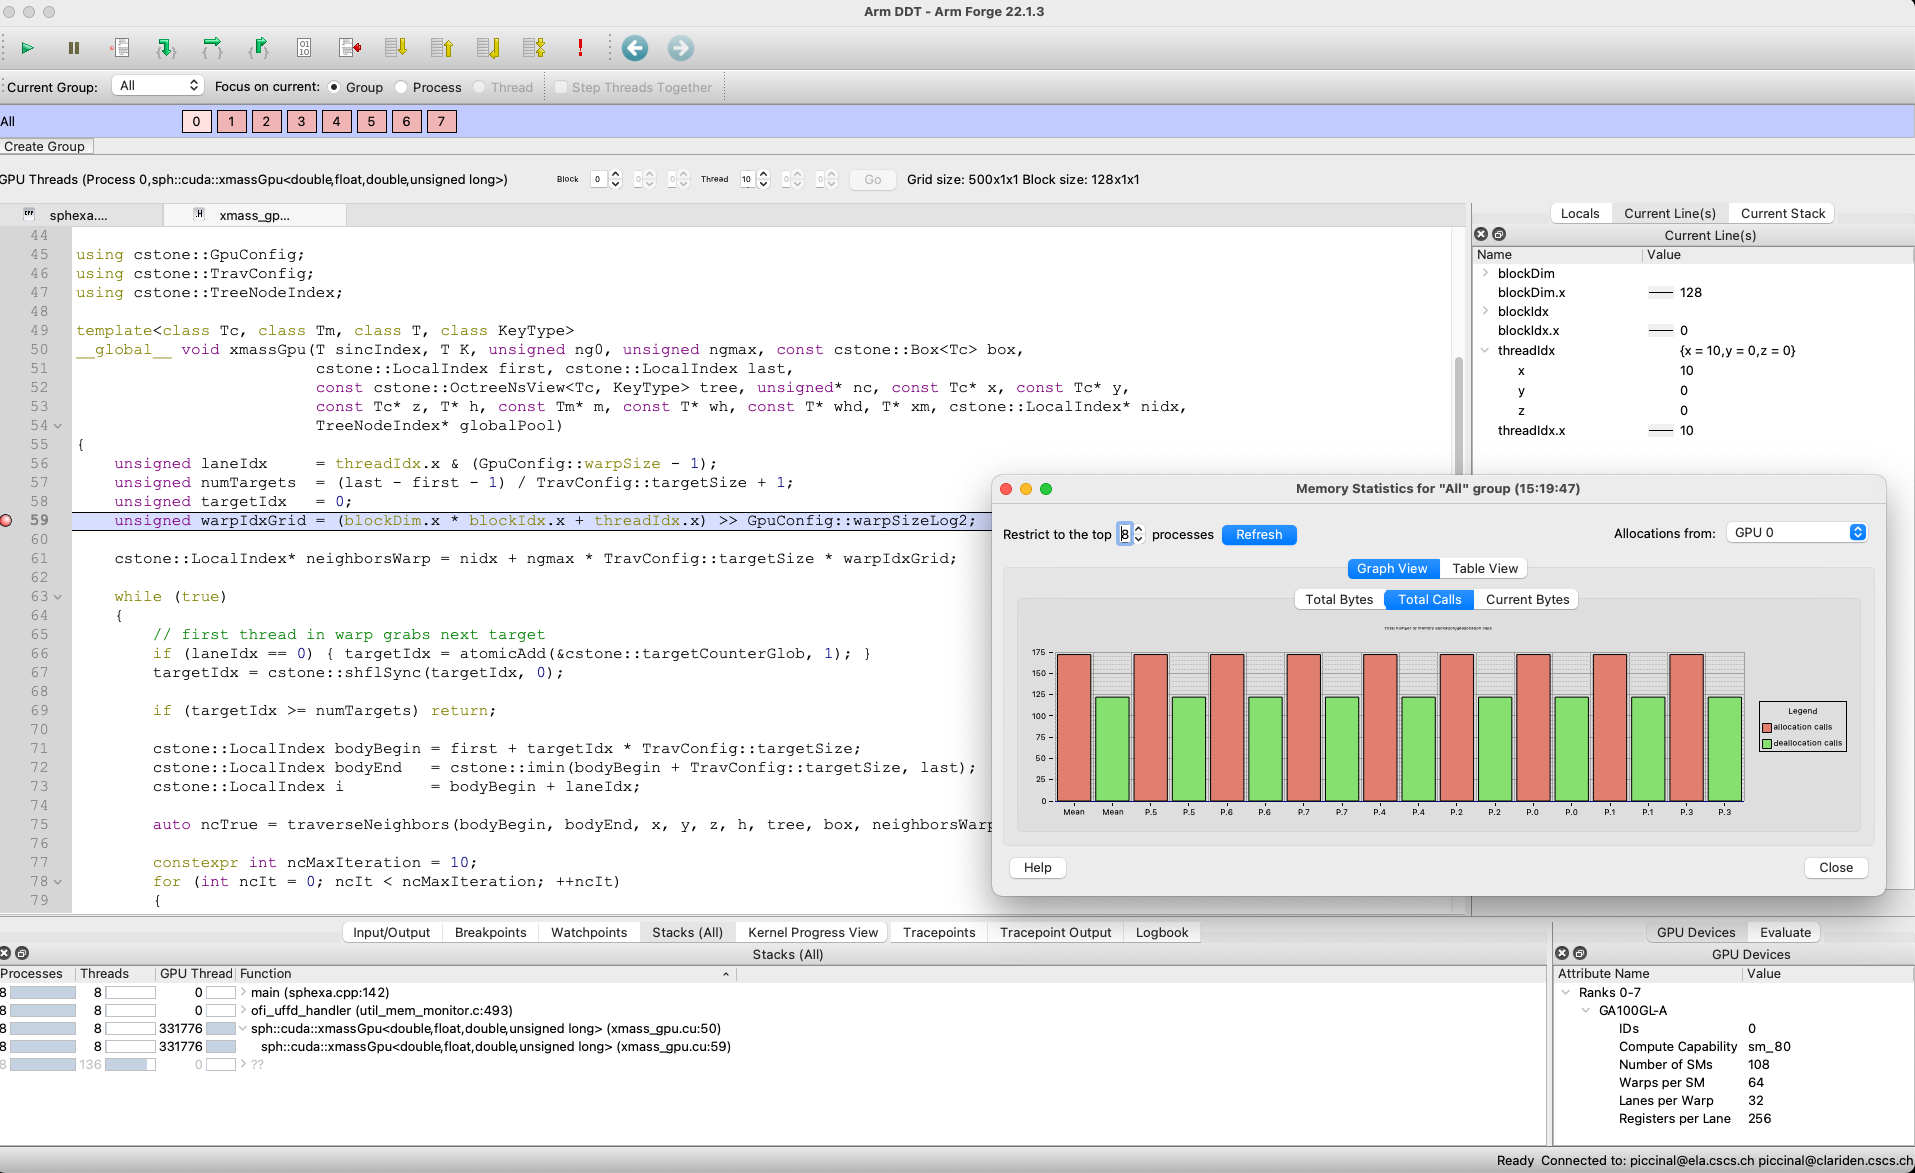
\includegraphics[width=\textwidth]{./images/sph-ddt-uenv.png}
    \end{center}
    \caption{Debugging SPH-EXA with Forge DDT.}
    \label{fig:sph-ddt-uenv}
\end{figure*}

This section focuses on showing the usage of the \href{https://www.linaroforge.com}{Forge DDT} debugger in a user-environment. 
% to help identifying bugs in MPI, OpenMP and Cuda/HIP codes.

Forge DDT can be launched using Express Launch (\lst{ddt srun myexe}), Reverse Connect (\lst{ddt --connect srun myexe}) or Offline mode (\lst{ddt --offline srun myexe}). 
Express Launch requires a good X11 connection hence it is recommended to use the Reverse Connect method, which uses the Remote Client to debug remote jobs while running the user interface on a local machine.
In addition, Forge DDT can be configured to integrate with queuing systems, allowing for the submission of jobs directly from the user interface.
The debugger can also open and debug one or more core files after an application terminates or attach to running programs.

In a classic workflow, users build a debug version of their code with the -g and -G compilation flags and submit a job with the sbatch slurm command.
For example, the \lst{native.slurm} script:
%
\lstinputlisting[language=bash]{src/ddt/native.slurm}
%
will load the Cray Programming Environment (CPE) and launch the debugger with the \lst{ddt --connect} command.
As the job starts, the users can use the remote client installed on their local machine to debug the code.

When running in a user-environment, it is required to manually launch the debugger.
For example, the \lst{uenv.slurm} script:
%
\lstinputlisting[language=bash]{src/ddt/uenv.slurm}
%
will mount the uenv-file, load the User Environment and launch the debugger with the \lst{forge-client} command.
Similarly to the previous case, users can debug the code when the job starts.
\fig{fig:sph-ddt-uenv} shows the Forge DDT remote client connected to a job running the SPH-EXA code.
DDT can be used to debug parallel programs in both scenarios.
Attaching to running programs with Forge DDT in a user environment requires additional testing as the process running the application and the Forge DDT process are not necessarily in the same namespace.

% -------------------------------
\subsubsection{Performance tools}

\begin{table}[htp!]
    \centering
    \pgfplotstabletypeset[
        precision=0,
        every head row/.style={before row=\toprule,after row=\midrule},
        col sep=space, columns={num-tasks, H2D-MB-max, D2H-MB-max, D2D-MB-max},
        columns/num-tasks/.style={column name=A100},
        columns/H2D-MB-max/.style={column name=H2D},
        columns/D2H-MB-max/.style={column name=D2H},
        columns/D2D-MB-max/.style={column name=D2D},
    ]
        {./data/sphexa/gpu/run-report-A100-64M-SQFS-cpe2302-NSYS.tbl}
    \caption{CUDA memcpy}
    \label{table:nsys-A100}
\end{table}

Table \ref{table:nsys-A100} shows the amount of CUDA memory copies (in MB) for the Sedov--Taylor test case.
The performance data was collected with the NVIDIA {Nsight Systems\footnote{\url{https://developer.nvidia.com/nsight-systems}}}  tool.
The transfer sizes (in MB) for Host to Device (H2D), Device to Host (D2H) and Device to Device (D2D) for simulations with uenv and without uenv (cpe only) are equal, demonstrating that the performance tool can be used in both scenarios.

\begin{figure}[htp!]
    \begin{center}
        \begin{tikzpicture}[
    /pgfplots/every axis/.style={
    ybar stacked, bar width=5pt, x=0.4cm, % space between bars
    ymax=100,
    legend pos=outer north east,
    xlabel=Nodes, xtick=data,
    ylabel={Runtime percentage}, 
    symbolic x coords={1,1.1, 2,2.1, 4,4.1, 8,8.1, 12,12.1},
    % legend style = {at={(0.5, 0.5)}, anchor=center},
    },
]

\begin{axis}[bar shift=-6pt]
    \addplot table[x=cn, y=usr_cpe] {data/sphexa/scorep/results-A100.tbl};
    \addplot table[x=cn, y=omp_cpe] {data/sphexa/scorep/results-A100.tbl};
    \addplot table[x=cn, y=mpi_cpe] {data/sphexa/scorep/results-A100.tbl};
    \addplot table[x=cn, y=com_cpe] {data/sphexa/scorep/results-A100.tbl};
\end{axis}

\begin{axis}[bar shift=0pt,hide axis]
    \addplot+[] table[x=cn, y=usr_uenv] {data/sphexa/scorep/results-A100.tbl};
    \addplot+[] table[x=cn, y=omp_uenv] {data/sphexa/scorep/results-A100.tbl};
    \addplot+[] table[x=cn, y=mpi_uenv] {data/sphexa/scorep/results-A100.tbl};
    \addplot+[] table[x=cn, y=com_uenv] {data/sphexa/scorep/results-A100.tbl};
    \legend{{\% USR: cpe, uenv}, {\% OMP: cpe, uenv}, {\% MPI: cpe, uenv}, {\% COM: cpe, uenv}}
\end{axis}
\end{tikzpicture}

    \end{center}
    \caption{Weak scaling profiling results on AMD EPYC 7A53 CPU nodes for SPH-EXA.}
    \label{fig:sph-weak-scorep}
\end{figure}

\fig{fig:sph-weak-scorep} shows profiling results for the Sedov--Taylor test case on CPU nodes.
The performance data was collected with the Score-P\footnote{\url{https://score-p.org}} tool (version 8.1).
The breakdown of the runtime into different regions such as USER, OpenMP and MPI demonstrates that the performance tool can be used in both environments.

% keep for reference: mpip
% \begin{table}[htp!]
%     \centering
%     \pgfplotstabletypeset[
%         precision=2,
%         every head row/.style={before row=\toprule,after row=\midrule},
%         col sep=space, columns={cn, pctmpi_cpe1, pctmpi_cpe2, pctmpi_uenv1, pctmpi_uenv2},
%         columns/pctmpi_cpe1/.style={column name=$\% CPE_{try1}$},
%         columns/pctmpi_cpe2/.style={column name=$\% CPE_{try2}$},
%         columns/pctmpi_uenv1/.style={column name=$\% UENV_{try1}$},
%         columns/pctmpi_uenv2/.style={column name=$\% UENV_{try2}$},
%     ]
%         {./data/sphexa/mpi/amdepyc_7a53-mpi.tbl}
%     \caption{MPI $\%$, AMD 7A53 cpu}
%     \label{table:mpi}
% \end{table}


%%%%%%%%%%%%%%%%%%%%%%%%%%%%%%%%%%%%%%%%%%%%%%%%%%%%%%%
\section{Future work}
%%%%%%%%%%%%%%%%%%%%%%%%%%%%%%%%%%%%%%%%%%%%%%%%%%%%%%%

The user-environmnents on Cray EX systems presented here is currently being used internally by CSCS software development teams, and by the MeteoSwiss in preparation for their next operational weather forecast system.
The service will be rolled out to external users of vCluster users over 2023, and there will be further development to extend features and provide a robust service.


% Column break - todo - move to where it will balance the columns on the last page.
\vfill\eject

The CI/CD pipeline is a high priority, with integration with the ReFrame testing framework to ensure that software stacks are corrent and performant.

We plan to provide a mechanism for the command line tools and Slurm plugin to mount multiple images -- for which the main motivating use case is providing debugger and profiler toolchains alongside programming stacks.

A command line tool that provides a singled interface for users to query, download and interact with environments is under development.

We will discuss collaboration with HPE to provide \craympich and other CPE software packages via Spack stacks, as well as extending our current experimental support for other MPI distributions on Cray EX.

Finally, while the tools are designed by CSCS and for use on Alps, we would welcome collaboration with other sites.


%\begin{figure*}[htp!]
%    \begin{center}
%            \begin{tikzpicture}[scale=1]
        \begin{axis} [
            height=6cm, width=17cm,
            xmin = 1, xmax = 12,
            ymax = 10, ymin=-10,
            %ytick={-30,-20,-10,0,10,20,30},
            xtick={1,2,3,4,5,6,7,8,9,10,11,12},
            xticklabels={1,2,3,4,5,6,7,8,9,10,11,12},
            %x tick label style={rotate=60,anchor=east},
            axis line style=very thick,
            ylabel=Relative Throughput (\%),
            xlabel=Nodes,
            %title=\large \bf GROMACS through
            legend style = {at={(0.95,0.05)}, anchor=south east},
            grid=major
        ]
            \addplot[color=green!40!black,mark=square*,mark options={fill=white}, very thick]
                table[x=nodes, y expr={(\thisrow{uenv-max}/\thisrow{cpe-max} - 1) * 100}] {./data/gromacs/hEGFRDimerPair.tbl};
            \addlegendentry{uenv/cpe}
        \end{axis}
    \end{tikzpicture}


%    \end{center}
%    \caption{Relative performance of GROMACS when built using spack stacks and CPE.}
%    \label{fig:osu}
%\end{figure*}

%\begin{figure*}[htp!]
%    \begin{center}
%            \begin{tikzpicture}[scale=1]
        \begin{loglogaxis} [
            height=6cm, width=8.5cm,
            xmin = 1, xmax = 4194304,
            ymax = 40000, ymin=0.1,
            ytick={0.1,1,10,100,1000,10000},
            yticklabels={0.1,1,10,100,1000,10000},
            xtick={1,2,4,8,16,32,64,128,256,512,1024,2048,4096,8192, 16384,  32768,  65536,  131072, 262144, 524288, 1048576, 2097152, 4194304},
            %xticklabels={1,2,4,8,16,32,64,128,256,512,1k,2k,4k,8k,16k,32k,64k,128k,256k,512k,1M,2M,4M},
            xticklabels={},
            x tick label style={rotate=60,anchor=east},
            axis line style=very thick,
            ylabel=Bandwidth (MB/s),
            %xlabel=Message Size,
            title=\large \bf osu\_p2p,
            legend style = {at={(0.95,0.05)}, anchor=south east},
            legend columns=2,
            legend style={/tikz/every even column/.append style={column sep=0.5cm}},
            grid=major,
            name=first plot,
        ]
            \addplot[color=green!40!black, very thick, densely dotted, forget plot]
                table[x=bytes, y=cpe-cpu-bw] {./data/osu/p2p.tbl};
            \addplot[color=orange!90!black, very thick, densely dotted, forget plot]
                table[x=bytes, y=sq-cpu-bw] {./data/osu/p2p.tbl};

            \addplot[color=green!40!black, very thick, forget plot]
                table[x=bytes, y=cpe-gpu-bw] {./data/osu/p2p.tbl};
            \addplot[color=orange!90!black, very thick, forget plot]
                table[x=bytes, y=sq-gpu-bw] {./data/osu/p2p.tbl};

            \addlegendimage{color=green!40!black, line width=5pt}
            \addlegendentry{CPE}

            \addlegendimage{very thick}
            \addlegendentry{A100 GPU}

            \addlegendimage{color=orange!90!black, line width=5pt, solid}
            \addlegendentry{uenv}

            \addlegendimage{very thick, densely dotted}
            \addlegendentry{Rome CPU}
        \end{loglogaxis}
        \begin{axis} [
            at=(first plot.south),
            anchor=north,
            xmode=log,
            height=3cm, width=8.5cm,
            xmin = 1, xmax = 4194304,
            ymax = 30, ymin=-10,
            %ymax = 2, ymin=-2,
            ytick={-10,0,10,20},
            xtick={1,2,4,8,16,32,64,128,256,512,1024,2048,4096,8192, 16384,  32768,  65536,  131072, 262144, 524288, 1048576, 2097152, 4194304},
            xticklabels={1,2,4,8,16,32,64,128,256,512,1k,2k,4k,8k,16k,32k,64k,128k,256k,512k,1M,2M,4M},
            x tick label style={rotate=60,anchor=east},
            axis line style=very thick,
            ylabel=\%,
            xlabel=Message Size,
            %title=\large \bf osu\_bw,
            legend style = {at={(0.95,0.05)}, anchor=south east},
            grid=major
        ]
            \addplot[color=black!40!black, thick, densely dotted]
                table[x=bytes, y expr={((\thisrow{sq-cpu-bw}/\thisrow{cpe-cpu-bw} - 1) * 100}] {./data/osu/p2p.tbl};
            \addplot[color=black!90!black, thick, solid]
                table[x=bytes, y expr={((\thisrow{sq-gpu-bw}/\thisrow{cpe-gpu-bw} - 1)*100}] {./data/osu/p2p.tbl};

        \end{axis}
    \end{tikzpicture}

%        \hfill
%        \newline
%            \begin{tikzpicture}[scale=1]
        \begin{loglogaxis} [
            height=6cm, width=8.5cm,
            xmin = 1, xmax = 4194304,
            ymax = 200, ymin=1,
            ytick={0.1,1,10,100,1000,10000},
            yticklabels={0.1,1,10,100,1000,10000},
            xtick={1,2,4,8,16,32,64,128,256,512,1024,2048,4096,8192, 16384,  32768,  65536,  131072, 262144, 524288, 1048576, 2097152, 4194304},
            %xticklabels={1,2,4,8,16,32,64,128,256,512,1k,2k,4k,8k,16k,32k,64k,128k,256k,512k,1M,2M,4M},
            xticklabels={},
            x tick label style={rotate=60,anchor=east},
            axis line style=very thick,
            ylabel=Latency ($\mu$s),
            %xlabel=Message Size,
            title=\large \bf osu\_p2p,
            legend style = {at={(0.05,0.95)}, anchor=north west},
            legend columns=2,
            legend style={/tikz/every even column/.append style={column sep=0.5cm}},
            grid=major,
            name=first plot,
        ]

            \addplot[color=green!40!black, very thick, densely dotted, forget plot]
                table[x=bytes, y=cpe-cpu-lat] {./data/osu/p2p.tbl};
            \addplot[color=orange!90!black, very thick, densely dotted, forget plot]
                table[x=bytes, y=sq-cpu-lat] {./data/osu/p2p.tbl};

            \addplot[color=green!40!black, very thick, forget plot]
                table[x=bytes, y=cpe-gpu-lat] {./data/osu/p2p.tbl};
            \addplot[color=orange!90!black, very thick, forget plot]
                table[x=bytes, y=sq-gpu-lat] {./data/osu/p2p.tbl};

            \addlegendimage{color=green!40!black, line width=5pt}
            \addlegendentry{CPE}

            \addlegendimage{very thick}
            \addlegendentry{A100 GPU}

            \addlegendimage{color=orange!90!black, line width=5pt, solid}
            \addlegendentry{uenv}

            \addlegendimage{very thick, densely dotted}
            \addlegendentry{Rome CPU}


        \end{loglogaxis}
        \begin{axis} [
            at=(first plot.south),
            anchor=north,
            xmode=log,
            height=3cm, width=8.5cm,
            xmin = 1, xmax = 4194304,
            %ymax = 1, ymin=-1,
            %ytick={-1,0},
            xtick={1,2,4,8,16,32,64,128,256,512,1024,2048,4096,8192, 16384,  32768,  65536,  131072, 262144, 524288, 1048576, 2097152, 4194304},
            xticklabels={1,2,4,8,16,32,64,128,256,512,1k,2k,4k,8k,16k,32k,64k,128k,256k,512k,1M,2M,4M},
            x tick label style={rotate=60,anchor=east},
            axis line style=very thick,
            ylabel=\%,
            xlabel=Message Size,
            %title=\large \bf osu\_bw,
            legend style = {at={(0.95,0.05)}, anchor=south east},
            grid=major
        ]
            \addplot[color=black!40!black, thick, densely dotted]
                table[x=bytes, y expr={((\thisrow{sq-cpu-lat}/\thisrow{cpe-cpu-lat} - 1) * 100}] {./data/osu/p2p.tbl};
            \addplot[color=black!90!black, thick, solid]
                table[x=bytes, y expr={((\thisrow{sq-gpu-lat}/\thisrow{cpe-gpu-lat} - 1) * 100}] {./data/osu/p2p.tbl};

        \end{axis}
    \end{tikzpicture}

%        \hfill
%        \newline
%            \begin{tikzpicture}[scale=1]
        \begin{loglogaxis} [
            height=6cm, width=17cm,
            xmin = 1, xmax = 4194304,
            ymax = 1200, ymin=10,
            %ytick={10,100,1000,10000},
            yticklabels={10,100,1000},
            xtick={1,2,4,8,16,32,64,128,256,512,1024,2048,4096,8192, 16384,  32768,  65536,  131072, 262144, 524288, 1048576, 2097152, 4194304},
            %xticklabels={1,2,4,8,16,32,64,128,256,512,1k,2k,4k,8k,16k,32k,64k,128k,256k,512k,1M,2M,4M},
            xticklabels={},
            x tick label style={rotate=60,anchor=east},
            axis line style=very thick,
            ylabel=Latency ($\mu$s),
            %xlabel=Message Size,
            title=\large \bf osu\_alltoall,
            legend style = {at={(0.05,0.95)}, anchor=north west},
            legend columns=2,
            legend style={/tikz/every even column/.append style={column sep=0.5cm}},
            grid=major,
            name=first plot,
        ]
            \addplot[color=green!40!black,mark=square*,mark options={fill opacity=0.0, solid, thick}, thin, densely dotted, forget plot]
                table[x=bytes, y=cpe-cpu] {./data/osu/all2all.tbl};
            %\addlegendentry{cpe/cpu - Rome CPU}
            \addplot[color=orange!90!black,mark=square*,mark options={fill opacity=0.0, solid, thick}, thin, densely dotted, forget plot]
                table[x=bytes, y=uenv-cpu] {./data/osu/all2all.tbl};
            %\addlegendentry{uenv/cpu - Rome CPU}

            \addplot[color=green!40!black,mark=*,mark options={fill opacity=0.0, solid}, thin, forget plot]
                table[x=bytes, y=cpe-gpu] {./data/osu/all2all.tbl};
            %\addlegendentry{cpe/gpu -- A100 GPU}
            \addplot[color=orange!90!black,mark=*,mark options={fill opacity=0.0, solid}, thin, forget plot]
                table[x=bytes, y=uenv-gpu] {./data/osu/all2all.tbl};
            %\addlegendentry{uenv/gpu -- A100 GPU}

            \addlegendimage{color=green!40!black, very thick}
            \addlegendentry{CPE}

            \addlegendimage{only marks, mark=*, mark options={scale=1.8, fill opacity=0.0, solid, thick}, thin}
            \addlegendentry{A100 GPU}

            \addlegendimage{color=orange!90!black, very thick, solid}
            \addlegendentry{uenv}

            \addlegendimage{only marks, mark=square*, mark options={scale=1.8, fill opacity=0.0, solid, thick}, thin, densely dotted}
            \addlegendentry{Rome CPU}
        \end{loglogaxis}
        \begin{axis} [
            at=(first plot.south),
            anchor=north,
            xmode=log,
            height=3cm, width=17cm,
            xmin = 1, xmax = 4194304,
            %ymax = 2, ymin=-2,
            %ytick={-2,-1,0,1},
            xtick={1,2,4,8,16,32,64,128,256,512,1024,2048,4096,8192, 16384,  32768,  65536,  131072, 262144, 524288, 1048576, 2097152, 4194304},
            xticklabels={1,2,4,8,16,32,64,128,256,512,1k,2k,4k,8k,16k,32k,64k,128k,256k,512k,1M,2M,4M},
            x tick label style={rotate=60,anchor=east},
            axis line style=very thick,
            ylabel=\%,
            xlabel=Message Size,
            %title=\large \bf osu\_bw,
            legend style = {at={(0.95,0.05)}, anchor=south east},
            grid=major
        ]
            \addplot[color=black!40!black,mark=square*,mark options={fill opacity=0.0, solid, thick}, thick, densely dotted]
                table[x=bytes, y expr={((\thisrow{uenv-cpu}/\thisrow{cpe-cpu} - 1) * 100}] {./data/osu/all2all.tbl};
            %\addlegendentry{uenv/cpe - Rome CPU}
            \addplot[color=black!90!black,mark=*,mark options={fill=white}, thick, solid]
                table[x=bytes, y expr={((\thisrow{uenv-gpu}/\thisrow{cpe-gpu} - 1) * 100}] {./data/osu/all2all.tbl};
            %\addlegendentry{uenv/cpe - A100 GPU}

        \end{axis}
    \end{tikzpicture}

%        \hfill
%        \newline
%    \end{center}
%    \caption{OSU benchmark results comparing cray-mpich performance when built using CPE and spack-stacks (uenv) for host-host (cpu) and device-device (gpu) configurations.}
%    \label{fig:osu}
%\end{figure*}

%%% Local Variables:
%%% TeX-master: "paper"
%%% End:
